\section{Evaluation}
\label{sec:eval}

Our evaluation answers six questions:
\begin{description}
\item[RQ1:] How often do clean verdicts depend on library flows that the analysis does not model?
\item[RQ2:] How many of these verdicts do priced receipts clear at a certified risk, compared with the alternatives?
\item[RQ3:] Does the guarantee hold when the answer key changes?
\item[RQ4:] What makes a pricer useful?
\item[RQ5:] Can checking a few receipt facts clear more verdicts?
\item[RQ6:] Does a threshold certified on benign apps hold on malware?
\end{description}

\subsection{Experimental Setup}
\label{sec:setup}

\paragraph{Apps.}
We downloaded about 580 open-source apps from F-Droid and built flow graphs for the 332 that fit our memory and time limits; 324 of them have at least one clean, hole-dependent sink.
These apps contain 79{,}847 clean, hole-dependent sinks whose status the main key decides; 20{,}104 of them never receive sensitive data.
We call these 20{,}104 sinks the \emph{hard slice}: they are leak-free, but a sound analysis cannot clear them.
For RQ6 we use TaintBench~\cite{taintbench}, 39 malware apps with 203 documented leaks; we built graphs for 33 of them.

\paragraph{Answer keys.}
A wrong clearance is defined relative to a key, so we use several keys built in different ways.
\begin{itemize}
\item The \emph{main key} uses FlowDroid's hand-written models where they exist. For the 12{,}274 methods FlowDroid does not model, it uses the labels on which two language models from different families, Sonnet~5 and GPT-6.1, agree when both are given the written definition of Section~\ref{sec:flow}; where they disagree, it uses K2 (below) if K2 decides the fact, and otherwise leaves the fact unknown.
\item The \emph{deletion keys} contain no language-model labels. They take FlowDroid's models as the truth and delete a share of the modeled classes; the deleted classes become priced holes, and all other modeled classes stay fixed. Deleting whole classes prevents a pricer from copying the answer of a sibling method.
\item \emph{K2} uses summaries that StubDroid~\cite{stubdroid} generates from the Android~13 and Java~8 source code.
\item The \emph{Sonnet} and \emph{GPT} keys label the unmodeled methods with one model each, asked a short question without the written definition.
\item The \emph{audited key} replaces the labels of the 446 facts that all accepted verdicts rest on by the answers of an audit, in which a person read the Android source code of 67 facts.
\end{itemize}

\paragraph{Protocol.}
We split the apps at random into two halves 200 times.
In each split, we certify a threshold on one half ($\varepsilon=0.1$, thresholds from 0.01 to 0.5) and measure two numbers on the other half: the share of the hard slice that is cleared, and the share of apps with at least one wrong clearance.
We report the means over the 200 splits.
The guarantee concerns the second number: it should stay below $\alpha$.

\subsection{RQ1: Dependence on Unmodeled Library Flows}
\label{sec:rq1}

To measure how much a taint analysis relies on library models, we ran FlowDroid on 80 F-Droid apps twice: with its models and without them.
Table~\ref{tab:fd-none} shows that without its models FlowDroid loses 82\% of the leaking sinks it reports, and finds no leak that it does not also find with them.
This is the extreme case of a missing model; in practice the models cover some methods and miss others.
In our corpus, 12{,}274 of the 17{,}830 library methods that lie on a source-to-sink path have no FlowDroid model, and 22\% of the leak-free sinks depend on some library flow, so a sound analysis cannot clear them.
The same holds for real leaks: of the 92 documented TaintBench leaks that our analysis reaches, 48 (52\%) are reachable only through a library flow it does not model.

The dependence is not specific to our analysis.
We gave FlowDroid holes as well: FlowDroid reads library behavior from summary files, so opening every hole means adding a summary with every candidate flow for each method it does not model.
On the 120 apps where all of FlowDroid's runs finished within 20 minutes, open holes add 58 reported sinks in 19 apps.
For 43 of them, switching off the hole methods on the reported paths and running FlowDroid again removes the sink, so FlowDroid itself confirms the receipt.

\begin{table}[t]
\caption{FlowDroid on 80 F-Droid apps with and without its library models: leaking sink methods it reports.}
\label{tab:fd-none}
\small
\begin{tabular}{@{}lrrrr@{}}
\toprule
Apps & Number & With models & Without & Lost without models\\
\midrule
Both runs complete & 52 & 46 & 6 & 40 (87\%)\\
One run stopped at its memory limit & 17 & 108 & 21 & 87 (81\%)\\
All apps with both answers & 69 & 154 & 27 & 127 (82\%)\\
\bottomrule
\end{tabular}
\end{table}

\answer{\textbf{RQ1:} Clean verdicts often depend on unmodeled library flows: 22\% of the leak-free sinks in our corpus and half of the reachable documented malware leaks do, and FlowDroid loses 82\% of its leaks without its library models.}

\subsection{RQ2: How Much Do Receipts Clear?}
\label{sec:rq2}

\begin{table}[t]
\caption{Share of the hard slice cleared at a certified threshold, and held-out apps with a wrong clearance (in brackets). Main key, 324 apps.}
\label{tab:main}
\small
\begin{tabular}{@{}lccc@{}}
\toprule
Pricer & $\alpha=0.10$ & $\alpha=0.05$ & $\alpha=0.02$\\
\midrule
Counting (receipt size) & 0\% & 0\% & 0\%\\
Frequency prior & 8.9\% (0.0\%) & 8.9\% (0.0\%) & --\\
Feature classifier & 43.8\% (4.7\%) & 28.8\% (0.5\%) & --\\
Sonnet~5 & 30.9\% (3.8\%) & 23.8\% (0.0\%) & --\\
Jev & 58.9\% (5.2\%) & 48.3\% (1.5\%) & 45.3\% (0.0\%)\\
\bottomrule
\end{tabular}
\end{table}

\begin{figure}[t]
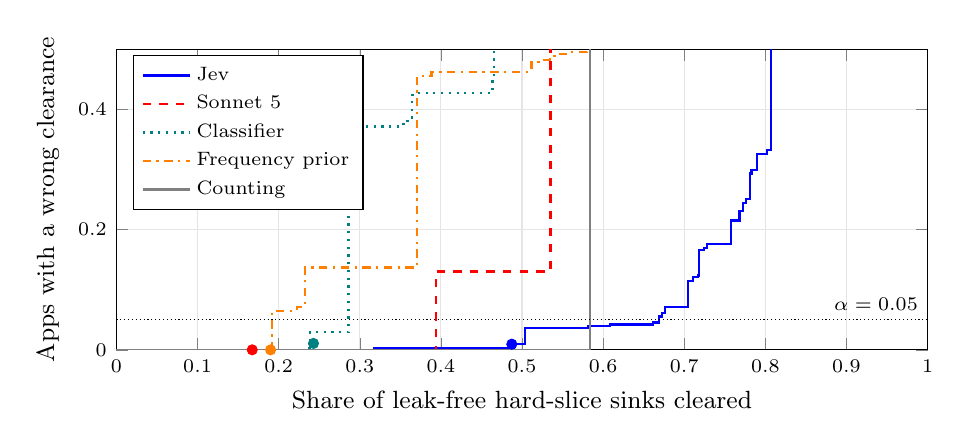
\begin{tikzpicture}
\begin{axis}[width=0.98\linewidth, height=5.4cm, xmin=0, xmax=1, ymin=0, ymax=0.5,
  xlabel={Share of leak-free hard-slice sinks cleared}, ylabel={Apps with a wrong clearance},
  legend style={font=\scriptsize, at={(0.02,0.98)}, anchor=north west}, legend cell align=left,
  tick label style={font=\scriptsize}, label style={font=\small}, grid=major, grid style={gray!20}]
\addplot[blue, thick, const plot mark left] coordinates {(0.0002,0.0000) (0.0605,0.0000) (0.0827,0.0000) (0.0921,0.0000) (0.1181,0.0000) (0.1841,0.0000) (0.1897,0.0000) (0.1965,0.0000) (0.2407,0.0000) (0.2520,0.0000) (0.2762,0.0000) (0.2994,0.0000) (0.3050,0.0000) (0.3118,0.0000) (0.3180,0.0033) (0.3261,0.0033) (0.3355,0.0033) (0.3520,0.0033) (0.3597,0.0033) (0.3755,0.0033) (0.4735,0.0033) (0.4902,0.0098) (0.5009,0.0098) (0.5032,0.0358) (0.5102,0.0358) (0.5233,0.0358) (0.5820,0.0391) (0.5871,0.0391) (0.5936,0.0391) (0.6010,0.0391) (0.6087,0.0423) (0.6149,0.0423) (0.6450,0.0423) (0.6527,0.0423) (0.6610,0.0456) (0.6685,0.0554) (0.6721,0.0619) (0.6760,0.0717) (0.7044,0.1140) (0.7110,0.1205) (0.7170,0.1238) (0.7185,0.1661) (0.7241,0.1694) (0.7285,0.1759) (0.7580,0.2150) (0.7666,0.2150) (0.7680,0.2313) (0.7728,0.2443) (0.7760,0.2508) (0.7802,0.2508) (0.7807,0.2932) (0.7830,0.2997) (0.7900,0.3257) (0.7994,0.3257) (0.8018,0.3322) (0.8065,0.8208) (0.8082,0.8274) (0.8133,0.8339) (0.8182,0.8339) (0.8347,0.8371) (0.8394,0.8534) (0.8469,0.8567) (0.8750,0.8567) (0.8798,0.8632) (0.8821,0.8697) (0.8847,0.8762) (0.8917,0.8827) (0.9022,0.8860) (0.9205,0.8860) (0.9270,0.8860) (0.9336,0.8860) (0.9522,0.8860) (0.9590,0.8860) (0.9665,0.8860) (0.9716,0.8860) (0.9774,0.8860) (0.9831,0.8893) (0.9878,0.8925) (0.9919,0.8958) (0.9955,0.9251) (1.0000,0.9349)};
\addlegendentry{Jev}
\addplot[red, thick, dashed, const plot mark left] coordinates {(0.0000,0.0000) (0.1674,0.0000) (0.3939,0.1303) (0.4285,0.1303) (0.5350,0.8078) (0.5918,0.8111) (0.6068,0.8111) (0.6350,0.8111) (0.6608,0.8111) (0.6805,0.8111) (0.6948,0.8404) (0.7063,0.8404) (0.7202,0.8436) (0.7305,0.8436) (0.7356,0.8436) (0.7433,0.8436) (0.8195,0.8436) (0.8274,0.8436) (0.8509,0.8436) (0.8554,0.8436) (0.8637,0.8436) (0.8687,0.8469) (0.8772,0.8469) (0.8823,0.8469) (0.9109,0.8469) (0.9184,0.8469) (0.9287,0.8534) (0.9332,0.8534) (0.9383,0.8534) (0.9545,0.8534) (0.9616,0.8567) (0.9902,0.8567) (0.9910,0.8664) (0.9987,0.8827) (0.9998,0.8925) (1.0000,0.9349)};
\addlegendentry{Sonnet~5}
\addplot[teal, thick, dotted, const plot mark left] coordinates {(0.0000,0.0000) (0.2307,0.0000) (0.2351,0.0033) (0.2382,0.0293) (0.2804,0.0293) (0.2862,0.0293) (0.2862,0.3648) (0.2879,0.3713) (0.3539,0.3811) (0.3637,0.3811) (0.3646,0.4235) (0.3693,0.4267) (0.3750,0.4267) (0.4184,0.4267) (0.4635,0.4528) (0.4650,0.5342) (0.4710,0.5342) (0.4754,0.5342) (0.4757,0.5440) (0.4819,0.5440) (0.5784,0.5472) (0.5829,0.5472) (0.5867,0.5570) (0.5920,0.5570) (0.6002,0.5668) (0.6049,0.5668) (0.6166,0.5668) (0.6190,0.5831) (0.6205,0.6026) (0.6252,0.6091) (0.6329,0.6091) (0.6401,0.6091) (0.6454,0.6091) (0.6516,0.6124) (0.7302,0.6124) (0.7382,0.6124) (0.7439,0.6124) (0.7456,0.6319) (0.7591,0.6352) (0.7649,0.6515) (0.7713,0.6515) (0.7806,0.6515) (0.7868,0.6515) (0.7909,0.6547) (0.8012,0.6547) (0.8041,0.6678) (0.8063,0.6808) (0.8084,0.7948) (0.8125,0.7948) (0.8197,0.7948) (0.8261,0.7980) (0.8304,0.8436) (0.8349,0.8436) (0.8413,0.8436) (0.8481,0.8436) (0.8541,0.8436) (0.8595,0.8502) (0.8637,0.8502) (0.8695,0.8502) (0.8744,0.8502) (0.8751,0.8599) (0.8825,0.8664) (0.8939,0.8664) (0.9022,0.8697) (0.9077,0.8697) (0.9107,0.8795) (0.9124,0.9023) (0.9259,0.9055) (0.9304,0.9088) (0.9387,0.9088) (0.9622,0.9088) (0.9667,0.9186) (0.9964,0.9186) (0.9977,0.9251) (1.0000,0.9349)};
\addlegendentry{Classifier}
\addplot[orange, thick, dashdotted, const plot mark left] coordinates {(0.0053,0.0000) (0.0651,0.0000) (0.0696,0.0000) (0.0754,0.0000) (0.1140,0.0000) (0.1841,0.0000) (0.1897,0.0000) (0.1922,0.0651) (0.2131,0.0651) (0.2228,0.0717) (0.2319,0.0717) (0.2320,0.1368) (0.3706,0.4560) (0.3795,0.4560) (0.3883,0.4625) (0.4882,0.4625) (0.5105,0.4625) (0.5109,0.4691) (0.5117,0.4788) (0.5220,0.4788) (0.5269,0.4821) (0.5342,0.4886) (0.5401,0.4919) (0.5476,0.4919) (0.5560,0.4951) (0.5799,0.5179) (0.5848,0.5179) (0.6408,0.5212) (0.6470,0.5212) (0.6502,0.5342) (0.6506,0.5407) (0.6566,0.5407) (0.6615,0.5440) (0.6642,0.6026) (0.6707,0.6026) (0.6794,0.6156) (0.6929,0.6156) (0.7021,0.6254) (0.7161,0.6254) (0.7194,0.6450) (0.7226,0.6580) (0.7268,0.6612) (0.7279,0.6678) (0.7381,0.6710) (0.7420,0.6775) (0.7488,0.7068) (0.7529,0.7068) (0.7563,0.7166) (0.7580,0.7655) (0.7621,0.7687) (0.7681,0.7785) (0.7736,0.7818) (0.7830,0.7915) (0.7901,0.8697) (0.7943,0.9088) (0.8409,0.9088) (0.8490,0.9088) (0.8556,0.9121) (0.8599,0.9121) (0.8881,0.9121) (0.8968,0.9121) (0.9011,0.9121) (0.9062,0.9186) (0.9127,0.9186) (0.9133,0.9251) (0.9186,0.9251) (0.9285,0.9251) (0.9383,0.9251) (0.9466,0.9251) (0.9603,0.9251) (0.9663,0.9283) (0.9712,0.9283) (0.9795,0.9283) (0.9846,0.9283) (0.9866,0.9349) (0.9919,0.9349) (0.9996,0.9349)};
\addlegendentry{Frequency prior}
\addplot[gray, thick, const plot mark left] coordinates {(0.0000,0.0000) (0.5835,0.8664) (0.7390,0.8860) (0.8466,0.8893) (0.8862,0.9283) (0.9041,0.9349) (0.9297,0.9349) (0.9440,0.9349) (0.9502,0.9349) (0.9720,0.9349) (0.9780,0.9349) (0.9851,0.9349) (0.9915,0.9349) (0.9968,0.9349)};
\addlegendentry{Counting}
\addplot[only marks, mark=*, mark size=1.8pt, blue, forget plot] coordinates {(0.4874,0.0094)};
\addplot[only marks, mark=*, mark size=1.8pt, red, forget plot] coordinates {(0.1674,0.0000)};
\addplot[only marks, mark=*, mark size=1.8pt, teal, forget plot] coordinates {(0.2429,0.0107)};
\addplot[only marks, mark=*, mark size=1.8pt, orange, forget plot] coordinates {(0.1900,0.0000)};
\addplot[black, densely dotted, forget plot] coordinates {(0,0.05) (1,0.05)};
\node[font=\scriptsize, anchor=south east] at (axis cs:1,0.05) {$\alpha=0.05$};
\end{axis}
\end{tikzpicture}

\caption{Wrong clearances against cleared share on all 324 apps as the threshold grows. Dots: certified operating points at $\alpha=0.05$ (mean over 200 splits).}
\label{fig:curve}
\end{figure}

Table~\ref{tab:main} gives the cleared share for each pricer, and Figure~\ref{fig:curve} the whole trade-off between clearing and wrong clearances.
With Jev's prices, receipts clear 48\% of the hard slice at $\alpha=0.05$, and 1.5\% of held-out apps receive a wrong clearance.
Together with the sinks a sound analysis already clears, 89\% of all leak-free sinks are cleared, against 78\% for the sound analysis alone.
In every row the observed error stays below $\alpha$, as Proposition~\ref{prop:ltt} predicts; what differs is how much is cleared.

\emph{Counting assumptions clears nothing.}
Counting gives every receipt of size one the same bound, so the first threshold already clears every one-fact receipt, and that puts a wrong clearance in 94\% of the apps.
The calibration therefore refuses every threshold.
Prices are what make receipts usable.

\emph{A language model's answer taken as fact has no risk control.}
Taking the model's yes/no answers as library models clears 80 to 90\% of the hard slice on the deletion keys, but 3.5\% of the apps receive a wrong clearance on average and up to 7.7\% in some runs, above a 5\% target in 9 of 18 runs.
There is one operating point, and its error cannot be chosen.

\emph{The unit of the guarantee matters.}
Table~\ref{tab:unit} compares our per-program calibration with conformal selection over verdicts~\cite{conformalselection}, which controls the share of wrong verdicts among the cleared ones.
At a 5\% target, conformal selection clears more, 73.5\%, but its wrong verdicts are spread over 192 of the 324 apps.
A user reading one app's report would see a wrong clearance more often than not.
Using the bound directly as a probability, without calibration, is safe for Jev but clears only 7.8\%, because its prices are conservative.
The certified result changes little with the confidence parameter, the size of the calibration half, or when apps that bundle the same libraries are kept on the same side of each split.
In a few splits the held-out share of wrong apps exceeds 5\%, as the bracket in Table~\ref{tab:unit} shows; the guarantee bounds how often this happens (at most a share $\varepsilon$ of calibrations), not each split.

\begin{table}[t]
\caption{Calibration unit and sensitivity (Jev, main key, $\alpha=0.05$). Brackets: 5th to 95th percentile over 200 splits.}
\label{tab:unit}
\small
\begin{tabular}{@{}lll@{}}
\toprule
Procedure & Cleared & Apps with a wrong clearance\\
\midrule
Bound used as a probability, $\delta=\alpha$ & 7.8\% & 0 of 324\\
Conformal selection over verdicts, 1\% / 5\% / 10\% & 71.2 / 73.5 / 76.1\% & 10 / 59 / 78\%\\
\midrule
Per program (ours), $\varepsilon=0.1$, 50\% calibration & 48.3\% [42.5, 57.6] & 1.5\% [0.0, 5.6]\\
\quad $\varepsilon=0.05$ / $0.2$ & 47.0 / 50.6\% & 0.9 / 2.4\%\\
\quad 30\% / 70\% of apps for calibration & 46.9 / 47.2\% & 0.7 / 1.2\%\\
\quad apps sharing libraries kept together & 46.6\% [43.0, 56.8] & 0.6\% [0.0, 5.3]\\
\bottomrule
\end{tabular}
\end{table}

\answer{\textbf{RQ2:} At a 5\% target, priced receipts clear 48\% of the leak-free sinks a sound analysis cannot clear, with wrong clearances in 1.5\% of held-out apps. Counting assumptions clears nothing, a language model taken as fact has no risk control, and per-verdict selection leaves wrong clearances in most apps.}

\subsection{RQ3: Robustness to the Answer Key}
\label{sec:rq3}

Every answer key can be wrong, so we repeat the calibration under each key in Table~\ref{tab:keys}.
The guarantee holds under all of them: the share of held-out apps with a wrong clearance stays at or below 2.6\% at $\alpha=0.05$.
The cleared share, however, depends on the key.
Keys that call more flows real leave fewer leak-free sinks and make each receipt more likely to contain a real flow.
Asked only a short question, GPT-6.1 calls 53\% of the candidate flows real against Sonnet's 35\%, and Jev's cleared share is 23\% under the GPT key against 40\% under the Sonnet key.
Flipping 11\% of the Sonnet key's ``no'' labels at random, the error rate a person's check of these labels suggested, has a similar effect.

\begin{table}[t]
\caption{Cleared share and held-out apps with a wrong clearance (in brackets) at $\alpha=0.05$ under other answer keys.}
\label{tab:keys}
\small
\begin{tabular}{@{}llll@{}}
\toprule
Key & Jev & Sonnet~5 & Feature classifier\\
\midrule
Main (two models agree) & 48.3\% (1.5\%) & 23.8\% (0.0\%) & 28.8\% (0.5\%)\\
Sonnet labels (short question) & 40.0\% (1.0\%) & 29.6\% (2.5\%) & 22.0\% (0.7\%)\\
Sonnet labels with audit answers & 39.4\% (2.0\%) & -- & --\\
K2 (StubDroid on Android code) & 25.7\% (1.7\%) & 33.6\% (2.3\%) & 20.4\% (2.3\%)\\
Deletion, 25\% of classes & 52.2\% (0.8\%) & 81.9\% (0.5\%) & 71.4\% (1.6\%)\\
Deletion, 75\% of classes & 50.9\% (1.3\%) & 79.1\% (1.0\%) & 33.1\% (0.5\%)\\
GPT labels & 22.9\% (1.8\%) & 24.0\% (0.9\%) & --\\
Noisy Sonnet key (3 draws) & 7.6--13.9\% ($\le$2.6\%) & 17.0--23.1\% ($\le$1.6\%) & --\\
\bottomrule
\end{tabular}
\end{table}

\emph{Is the key independent of the pricer?}
Sonnet~5 is both a pricer and one of the two labelers of the main key.
Under the keys that contain no Sonnet labels, the deletion keys, K2 and the GPT key, Sonnet is as good as or better than Jev, so agreement with itself does not explain its results; under the Sonnet-only key it does better than under the main key, which is why we do not use that key as the main one.

\emph{Does the key follow the definition?}
The disagreement between Sonnet and GPT comes from the question, not from the models.
Asked the short question, the two models agree on 81\% of the candidate flows (Cohen's $\kappa=0.62$), and they agree with a person's source-code checks on 81\% and 90\% of the facts.
Asked again with the written definition and one reason code per answer (Appendix~\ref{app:flow}), they agree on 90\% of 37{,}160 candidate flows ($\kappa=0.80$), both call about 41\% of the flows real, and they agree with the person on 92\% and 93\% of the 60 facts; on the 57 facts where both models give the same answer, the person agrees with that answer 54 times (95\%).
This is why the main key uses the answers on which both models agree under the written definition.

\emph{The deletion keys test pricers on code they have not seen.}
Figure~\ref{fig:deletion} shows the cleared share as more classes are deleted.
A classifier trained on FlowDroid's models is strong when single methods are deleted, because it learns the conventions of the remaining sibling methods, and collapses when whole classes are deleted, which is the realistic case: 86\% of the unmodeled methods that appear in receipts belong to classes FlowDroid does not model at all.
Language-model pricers do not depend on siblings and keep their clearance.

\begin{figure}[t]
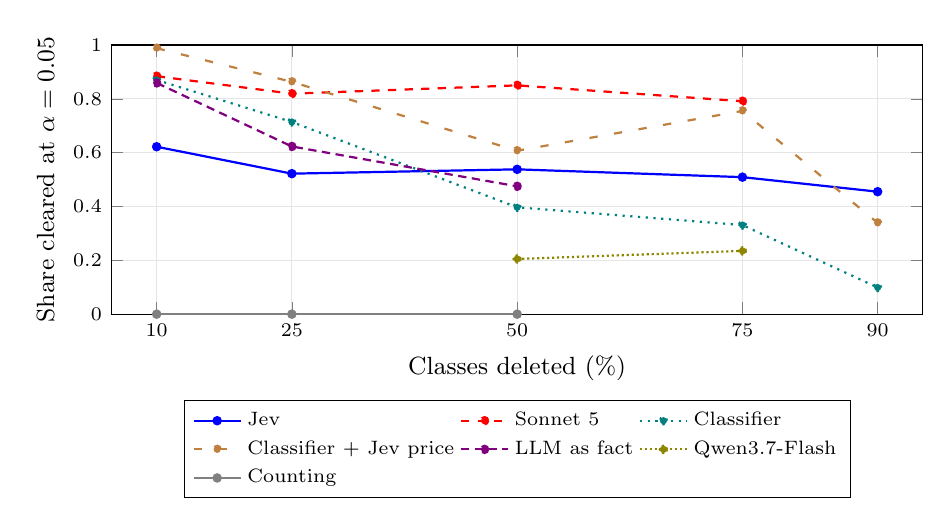
\begin{tikzpicture}
\begin{axis}[width=0.98\linewidth, height=5cm, xmin=5, xmax=95, ymin=0, ymax=1,
  xlabel={Classes deleted (\%)}, ylabel={Share cleared at $\alpha=0.05$}, xtick={10,25,50,75,90},
  legend style={font=\scriptsize, at={(0.5,-0.32)}, anchor=north}, legend cell align=left, legend columns=3,
  tick label style={font=\scriptsize}, label style={font=\small}, grid=major, grid style={gray!20}]
\addplot[blue, thick, mark=*, mark size=1.3pt] coordinates {(10,0.6220) (25,0.5220) (50,0.5380) (75,0.5090) (90,0.4550)};
\addlegendentry{Jev}
\addplot[red, thick, dashed, mark=*, mark size=1.3pt] coordinates {(10,0.8840) (25,0.8190) (50,0.8500) (75,0.7910)};
\addlegendentry{Sonnet~5}
\addplot[teal, thick, dotted, mark=*, mark size=1.3pt] coordinates {(10,0.8700) (25,0.7140) (50,0.3970) (75,0.3310) (90,0.0990)};
\addlegendentry{Classifier}
\addplot[brown, thick, loosely dashed, mark=*, mark size=1.3pt] coordinates {(10,0.9880) (25,0.8630) (50,0.6070) (75,0.7550) (90,0.3390)};
\addlegendentry{Classifier + Jev price}
\addplot[violet, thick, densely dashed, mark=*, mark size=1.3pt] coordinates {(10,0.8590) (25,0.6230) (50,0.4750)};
\addlegendentry{LLM as fact}
\addplot[olive, thick, densely dotted, mark=*, mark size=1.3pt] coordinates {(50,0.2050) (75,0.2350)};
\addlegendentry{Qwen3.7-Flash}
\addplot[gray, thick, mark=*, mark size=1.3pt] coordinates {(10,0.0000) (25,0.0000) (50,0.0000)};
\addlegendentry{Counting}
\end{axis}
\end{tikzpicture}

\caption{Deletion keys: share of the hard slice cleared at $\alpha=0.05$ as more of FlowDroid's modeled classes are deleted (three seeds). In every cell, the share of calibrations whose held-out error exceeds $\alpha$ stays within $\varepsilon$.}
\label{fig:deletion}
\end{figure}

\answer{\textbf{RQ3:} The guarantee holds under all eight keys, including keys with no language-model labels and a key with random label noise. The cleared share depends on how many flows the key calls real; with the written definition, two model families agree with each other ($\kappa=0.80$), and where they agree, with a person's source checks (95\%).}

\subsection{RQ4: What Makes a Pricer Useful?}
\label{sec:rq4}

\begin{table}[t]
\caption{Pricers on the main key (200 half splits). Certified: number of splits in which a threshold was certified; cleared: mean over those splits. Price: whole corpus.}
\label{tab:panel}
\small
\begin{tabular}{@{}lrll@{}}
\toprule
Pricer & Price & $\alpha=0.05$: certified, cleared & $\alpha=0.10$: certified, cleared\\
\midrule
Jev & \$0.4 & 200, 48.3\% & 200, 58.9\%\\
Sonnet~5 & \$16.4 & 200, 23.8\% & 200, 30.9\%\\
Qwen3.7-Flash & \$0.19 & 4, 30.3\% & 154, 30.3\%\\
Gemini-3.5-Flash-Lite & \$2.82 & 0 & 2, 21.0\%\\
DeepSeek-V4-Flash & \$0.37 & 0 & 0\\
Qwen3.8-27B & \$1.96 & 200, 0\% & 200, 0\%\\
GPT-5.6-luna & \$5.13 & 200, 4.2\% & 200, 4.2\%\\
\bottomrule
\end{tabular}
\end{table}

Table~\ref{tab:panel} adds five cheaper language models, asked the same question as Sonnet.
None of them clears much, and the reason is visible in their prices: they answer almost only with extreme values (Qwen3.8-27B gives 0.02 or 0.95 to 97\% of the flows) and give the lowest price to some real flows.
The lowest threshold that clears anything then already puts a wrong clearance in many apps, and the calibration refuses it.
The guarantee still holds: a poor pricer costs clearance, not validity.

\emph{Average ranking quality is not what counts.}
Table~\ref{tab:rank} shows that the classifier and Sonnet rank verdicts better than Jev on average (AUROC 0.981 and 0.964 against 0.935), yet clear much less at $\alpha=0.05$.
By Proposition~\ref{prop:order}, only the order of the bounds matters, and only at the low end, where verdicts are cleared: one real flow with a low price is enough to make an app wrong.
A pricer for receipts should be judged by its curve near the origin of Figure~\ref{fig:curve}, not by an average score.

\begin{table}[t]
\caption{Ranking quality (AUROC of the bound, real flows against leak-free sinks) and certified clearance over 200 half splits.}
\label{tab:rank}
\small
\begin{tabular}{@{}llrrrr@{}}
\toprule
Key & Pricer & AUROC & Cleared, $\alpha{=}0.05$ & Wrong, mean / p95 & Cleared, $\alpha{=}0.10$\\
\midrule
Main key & Jev & 0.970 & 48.7\% & 0.9\% / 5.8\% & 59.9\%\\
 & Sonnet~5 & 0.950 & 16.7\% & 0.0\% / 0.0\% & 16.6\%\\
 & Classifier & 0.965 & 24.3\% & 1.1\% / 4.5\% & 27.9\%\\
 & Frequency prior & 0.932 & 19.0\% & 0.0\% / 0.0\% & 18.8\%\\
 & Counting & 0.848 & 0.0\% & 0.0\% / 0.0\% & 0.0\%\\
\midrule
K2 (code-derived) & Jev & 0.999 & 93.1\% & 1.3\% / 3.1\% & 94.0\%\\
 & Sonnet~5 & 0.997 & 95.9\% & 1.6\% / 3.8\% & 96.5\%\\
 & Classifier & 0.998 & 42.5\% & 1.5\% / 6.1\% & 90.8\%\\
\bottomrule
\end{tabular}

\end{table}

\emph{Stating the flow rule in the question matters.}
Jev's clearance at $\alpha=0.05$ is 14.2\% when asked only whether a flow exists, 25.4\% when asked whether taint propagates, and 40.0\% when the question states that a tainted object taints everything read from it.
Without the rule, getters on tainted objects receive low prices, and the few real flows among them block the threshold.

\emph{How prices are combined matters less.}
With the same receipts, summing over distinct facts instead of edges clears 52.9\%, the largest single price 42.2\%, and the product under independence 54.2\%, all with at most 2.1\% of apps wrong.
The calibration makes each of these valid; the union bound is the one that is also a guaranteed upper bound for each verdict.

\answer{\textbf{RQ4:} A useful pricer gives low prices only to flows that are really absent. Jev clears 48 to 59\% of the hard slice and Sonnet~5 24 to 31\%; cheaper models answer too confidently and clear little, without breaking the guarantee. Stating the flow rule in the question nearly triples Jev's clearance.}

\subsection{RQ5: Checking Receipt Facts}
\label{sec:rq5}

\begin{table}[t]
\caption{Checking the top-ranked receipt facts (Jev, $\alpha=0.05$). Cleared: share of the original hard slice cleared, either because the sink no longer depends on any hole or because its new bound is accepted. Reported leaks: real flows the analysis now reports without holes.}
\label{tab:verify}
\small
\begin{tabular}{@{}llrrr@{}}
\toprule
Key & Facts checked & Cleared & Apps wrong & Reported real leaks\\
\midrule
Main & 0 & 46.9\% & 1.0\% & 12{,}152\\
 & 25, ranked by unlock & 64.6\% & 1.2\% & 26{,}901\\
 & 100, ranked by unlock & 72.9\% & 0.7\% & 33{,}179\\
 & 25, ranked by count & 49.0\% & 1.2\% & 26{,}292\\
 & 100, ranked by count & 68.4\% & 0.7\% & 34{,}788\\
 & 400, ranked by count & 83.0\% & 0.4\% & 40{,}485\\
 & 100, at random & 47.3\% & 1.0\% & 12{,}253\\
\midrule
K2 & 0 & 25.5\% & 1.7\% & 12{,}152\\
 & 50 & 78.7\% & 1.8\% & 13{,}441\\
 & 200 & 83.5\% & 0.9\% & 13{,}963\\
\bottomrule
\end{tabular}
\end{table}

A receipt fact often appears in many receipts; \texttt{Messenger.send} alone appears in the receipts of 481 accepted verdicts in 85 apps.
We therefore ask how much a person, or a test, gains by checking a few facts.
We rank facts without looking at any answer (Section~\ref{sec:verify}), let the key answer the top $K$, and certify the threshold again.
Table~\ref{tab:verify} shows the result.
Checking the 25 facts that would clear the most verdicts with a ``no'' (the unlock rule) raises the cleared share from 47\% to 65\% and doubles the number of real leaks the analysis reports, because a ``yes'' turns a library flow into a known flow.
With 100 checks the share reaches 73\%, and with 400 checks ranked by count, 83\%.
Checking 100 facts chosen at random changes nothing, so the ranking is what makes the checks useful.
Under the Sonnet key the order of the two rules is reversed: counting the uncleared verdicts a fact blocks works better there (64\% against 58\% at 100 checks), because more of the frequent facts are flows that the checks confirm.
The held-out error stays below the target in every row.

\answer{\textbf{RQ5:} Receipts make checking efficient: 25 well-chosen facts raise the cleared share from 47\% to 65\% and double the real leaks reported, while 100 random facts change nothing.}

\subsection{RQ6: Transfer to Malware}
\label{sec:rq6}

Our calibration apps are benign F-Droid apps, while a tool may be used on very different apps.
We therefore certify a threshold on all 324 F-Droid apps and apply it to the TaintBench malware apps.
For each documented leak, we look up our verdicts for the method that contains its sink (Table~\ref{tab:taintbench}).

\begin{table}[t]
\caption{TaintBench: documented leaks against our verdicts, and the threshold certified on the 324 F-Droid apps applied to the 31 malware apps with hole-dependent verdicts.}
\label{tab:taintbench}
\small
\begin{tabular}{@{}lr@{}}
\toprule
Documented leaks & 203\\
\quad outside our scope (no graph: 24; sink not in the list: 4) & 28\\
\quad reported without any library flow & 44\\
\quad reachable only through unmodeled library flows & 48\\
\quad not reached & 83\\
\midrule
Documented leaks cleared, Jev ($\delta=0.2$) / Sonnet~5 ($\delta=0.02$) & 3 / 3\\
Apps with a wrong clearance (main key), Jev / Sonnet~5 & 0 / 0 of 31\\
Leak-free hole-dependent verdicts cleared, Jev / Sonnet~5 & 31.5\% / 18.2\%\\
Counting, receipts of one fact: documented leaks cleared; apps wrong & 22; 21 of 31\\
\bottomrule
\end{tabular}
\end{table}

The threshold transfers: with Jev's and with Sonnet's prices, no malware app receives a wrong clearance by our key, and Jev clears 32\% of the leak-free hole-dependent verdicts.
Three documented leaks are cleared by both pricers.
All three are in one app and rest on one fact, \texttt{WebView.addJavascriptInterface} from receiver to argument.
The app registers an object whose methods return the device identifier, and the leak happens when JavaScript in the web page calls these methods.
That is a callback, which our flow definition excludes, so the key labels the fact ``no''.
The receipt shows exactly which assumption the three clearances share, so a user who disagrees with the definition can check this one fact.
Counting assumptions, in contrast, would clear 22 documented leaks.

\answer{\textbf{RQ6:} A threshold certified on benign apps held on 31 malware apps: no app received a wrong clearance with either pricer. The three documented leaks that were cleared all rest on one checkable fact about a callback.}
